\subsection{The ‘class’ Comment}\label{sec:ClassComment}
The documentation comment for a class\index{class}, an interface\index{interface}, an \lstinline|enum|\index{enum}, a record\index{record} or an annotation\index{annotation} (the \bsq{class comment}) describes that class, its purpose and its usage. If the class is not \lstinline|final|, the comment should provide some hints what the mount points\index{mount point}\footnote{Another term for \bdq{mount point} is \bdq{extension point}\index{extension point|see {mount point}}, but I do not like this expression as we do not always \textit{extend} a class on these points. Most often we replace existing behaviour to customise the class to our needs.} are and how to utilise them.

Then the class comment should list the authors of the class, using the \nameref{sec:TagAuthor}\index{author@"@author} tag, the class version (using the \nameref{sec:TagVersion}\index{version@"@version} tag), and when the class was added to the project with the \nameref{sec:TagSince}\index{since@"@since} tag, although this is optional if the information is already given within the package comment.

In case of a parameterized type\index{parameterized type} (a \bsq{generic}), the class comment must contain a \nameref{sec:TagParam}\index{param@"@param} tag for each formal parameter.

\keeplisting{17}
Here a real life sample for an interface\index{interface}
\begin{lstlisting}
/**
 *  <p>{@summary This is the basic interface for any kind of DAO 
 *  (Data Access Object).} It is based on sample code from the book 
 *  &quot;Java Persistence with Hibernate&quot;.</p>
 *
 *  @param  <T> The entity type for the DAO.
 *  @param  <I> The type of the entity id.
 *
 *  @author Thomas Thrien - thomas.thrien@tquadrat.org
 *  @version 2.3.4
 *  @since 1.2.3
 */
public interface GenericDAO<T,I>
{
    …
}   //  interface GenericDAO
\end{lstlisting}

The version information for the \nameref{sec:TagVersion}\index{version@"@version} tag (line~10) should be a reference to the version in the SCCS\index{SCCS}; if you are using Subversion\index{Subversion}, that line would look like this:
\begin{lstlisting}[firstnumber=9,language=Comment]
 …
 *  @version $Id:$
 …
\end{lstlisting}

The string \verb#$Id:$# will be replaced during checkin with information provided by Subversion\index{Subversion} if \bdq{\textit{keyword replacement}} is enabled. git\index{git} does not provide something similar out-of-the-box.

The class comment for a record\index{record} is a bit special as it has to incorporate the documentation for the record components (the fields of the record) as well as that for the constructor parameters (as both are the same). You use the \nameref{sec:TagParam}\index{param@"@param} tag for that.

The declaration for a record\index{record} \lstinline|Tupel| is shown below. Although not explicitly declared, the record\index{record} class has~…
\begin{itemize}[nosep]
	\item{…~a constructor\index{constructor}:
\keeplisting{4}
\begin{lstlisting}
public Tupel( final K key, final V value )
{
    this.key = key;
    this.value = value;
}
\end{lstlisting}}

	\item{…~the two attributes \bdq{\lstinline|public final K key|} and \bdq{\lstinline|public final V value|}}

	\item{
	\keeplisting{2}
	…~the two accessor methods\index{method!accessor method}:
\begin{lstlisting}
public final K key() { return key; }
public final V value() { return value; }
\end{lstlisting}}

	\item{…~and implementations for the methods \bdq{\lstinline|equals()|}, \bdq{\lstinline|hashCode()|} and \bdq{\lstinline|toString()|}}
\end{itemize}

The documentation for these elements is generated either based on the arguments for the \nameref{sec:TagParam} tags (see lines~13 and 14) or from standard texts.

\begin{lstlisting}[caption={A tupel class}]
/**
 *  <p>{@summary A tupel.} The first entry, usually referred to as 
 *  the &quot;key&quot; identifies the object, the second one is the
 *  &quot;value&quot;.</p>
 *  <p>The sort order is determined only through the keys, therefore
 *  {@link #compareTo(Tupel)}
 *  is not consistent with
 *  {@link #equals(Object)}.</p>
 *
 *  @param  <K> The type of the key.
 *  @param  <V> The type of the value.
 *
 *  @param  key The key of the tupel; can be {@code null}.
 *  @param  value   The value of the tupel; can be {@code null}.
 *
 *  @author Thomas Thrien - thomas.thrien@tquadrat.org
 *  @version $Id:$
 *  @since 1.2.3
 */
public record Tupel<K extends Comparable<K>,V>( K key, V value ) implements Comparable<Tupel<K,V>>
{
        /*---------*\
    ====** Methods **================================================
        \*---------*/
    /**
     *  {@inheritDoc} 
     */
    @Override
    public final int compareTo( final Tupel<K,V> o )
    {
        final var retValue = Comparator.comparing( Tupel<K,V>::key )
            .compare( this, o ); 

        //---* Done *------------------------------------------------
        return retValue;
    }   //  compareTo()
}
//  record Tupel
\end{lstlisting}
\clearpage
This is the first part of the class documentation, generated by the Javadoc\index{javadoc} tool from the source code above:
\begin{center}
	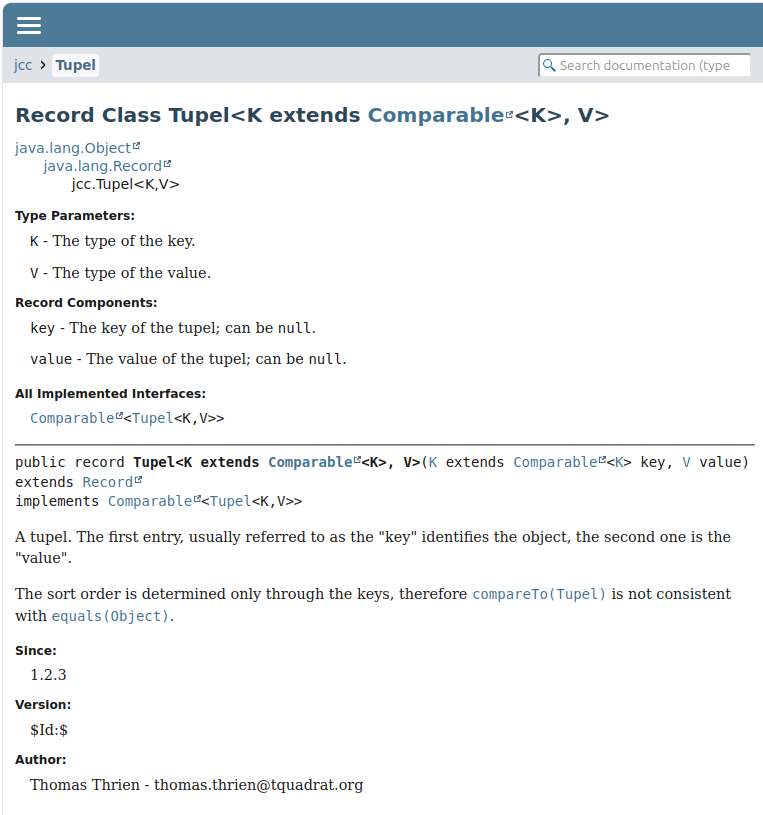
\includegraphics[scale=0.55]{comments/JavadocTupel1}
\end{center}

\clearpage
Despite none of the methods\index{method} nor the constructor\index{constructor} were explicitly defined, they are listed for the \lstinline|Tupel| record class\index{record}, even with a meaningful description:
\begin{center}
	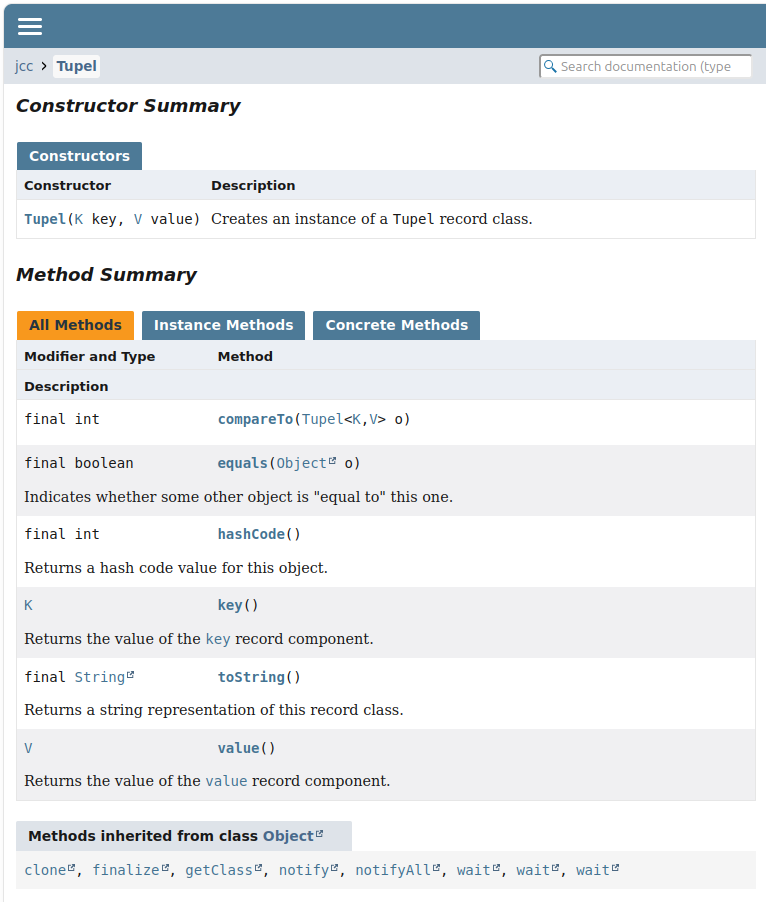
\includegraphics[scale=0.55]{comments/JavadocTupel2}
\end{center}
That there is no description for \lstinline|compareTo()| is due to a bug in the Javadoc tool in the version used for the generation; usually, the documentation is inherited from the overridden method\index{method!overridden method}. At the very least, the Javadoc tool\index{javadoc} generated the link to the documentation of the overridden method\index{method!overridden method} within the method's detailed documentation:
\begin{center}
	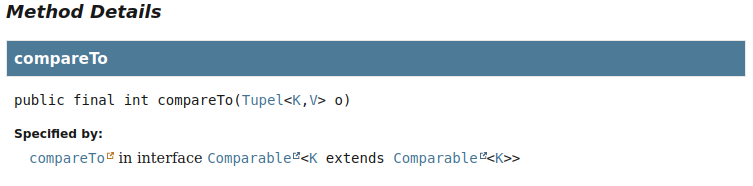
\includegraphics[scale=0.55]{comments/JavadocTupel3}
\end{center}

%==============================================================================
% End of file!!
%==============================================================================
